\documentclass{article}
\usepackage{graphicx}
\usepackage{authblk}
\usepackage{listings}
\usepackage{xcolor}
\usepackage[a4paper,
            bindingoffset=0.2in,
            left=0.5in,
            right=0.5in,
            top=0.5in,
            bottom=0.5in,
            footskip=.25in]{geometry}

\definecolor{mGreen}{rgb}{0,0.6,0}
\definecolor{mGray}{rgb}{0.5,0.5,0.5}
\definecolor{mPurple}{rgb}{0.58,0,0.82}
\definecolor{backgroundColour}{rgb}{0.95,0.95,0.92}

\lstdefinestyle{CStyle}{
	backgroundcolor=\color{backgroundColour},   
    commentstyle=\color{mGreen},
    keywordstyle=\color{magenta},
    numberstyle=\tiny\color{mGray},
    stringstyle=\color{mPurple},
    basicstyle=\footnotesize,
    breakatwhitespace=false,         
    breaklines=true,                 
    captionpos=b,                    
    keepspaces=true,                 
    numbers=left,                    
    numbersep=5pt,                  
    showspaces=false,                
    showstringspaces=false,
    showtabs=false,                  
    tabsize=2,
    language=C
}


\title{Assignment \#2 - Selection and Repetition}
\author{Cody Raposa}
\affil{ELEC2850 Microcontrollers Using C Programming}

\begin{document}
\maketitle
\begin{flushleft}
	\section{Q1 Code}
	\lstinputlisting[style=CStyle]{Q1.c}
    \begin{figure}[!h]
        \begin{centering}
          
\includegraphics[scale=1]{Q1_p1.png}
          \caption{Output for test case 9:30}
        \end{centering}
      \end{figure}
      \begin{figure}[!h]
        \begin{centering}
          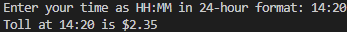
\includegraphics[scale=1]{Q1_p2.png}
          \caption{Output for test case 14:20}
        \end{centering}
      \end{figure}
      \newpage
    \section{Q2 Code}
    \lstinputlisting[style=CStyle]{Q2.c}
    \begin{figure}[!h]
        \begin{centering}
          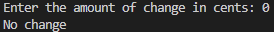
\includegraphics[scale=1]{Q2_p1.png}
          \caption{Output for test case 0}
        \end{centering}
      \end{figure}
    \begin{figure}[!h]
        \begin{centering}
          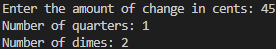
\includegraphics[scale=1]{Q2_p2.png}
          \caption{Output for test case 45}
        \end{centering}
      \end{figure}
    \begin{figure}[!h]
        \begin{centering}
          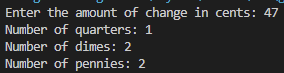
\includegraphics[scale=1]{Q2_p3.png}
          \caption{Output for test case 47}
        \end{centering}
    \end{figure}
    \newpage
    \section{Q3 Code}
    \lstinputlisting[style=CStyle]{Q3.c}
    \begin{figure}[!h]
        \begin{centering}
          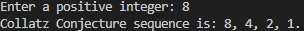
\includegraphics[scale=1]{Q3_p1.png}
          \caption{Output for test case 8}
        \end{centering}
      \end{figure}
    \begin{figure}[!h]
        \begin{centering}
          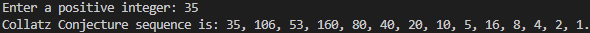
\includegraphics[scale=1]{Q3_p2.png}
          \caption{Output for test case 35}
        \end{centering}
    \end{figure}
\end{flushleft}
\end{document}